\documentclass[12pt]{report}
\usepackage[utf8]{inputenc}
\usepackage[T1]{fontenc}
\usepackage{german}
\usepackage{geometry}                % See geometry.pdf to learn the layout options. There are lots.
\geometry{a4paper}                   % ... or a4paper or a5paper or ... 
\usepackage[parfill]{parskip}    % Activate to begin paragraphs with an empty line rather than an indent
\usepackage{xifthen}
\usepackage{xstring}			% to check content of strings in xifthen
\usepackage{graphicx}
\usepackage[usenames,dvipsnames,table]{xcolor}
\usepackage{amssymb}
\usepackage{epstopdf}
\usepackage{hyperref}
\usepackage{fancyhdr}


\IfStrEq*{\languagename}{english}
	{
		\newcommand{\dalabel}{Diploma Thesis}
		\newcommand{\submittedlabel}{Submitted by}
		\newcommand{\datelabel}{Date}
		\newcommand{\supervisorlabel}{Supervisor}
		\newcommand{\projectpartnerlabel}{Project Partner}
	}
	{
		\newcommand{\dalabel}{Diplomarbeit}
		\newcommand{\submittedlabel}{Eingereicht von}
		\newcommand{\datelabel}{Datum}
		\newcommand{\supervisorlabel}{Betreuer}
		\newcommand{\projectpartnerlabel}{Projektpartner}
	}
 % This file should not really be touched
\newcommand{\titleofthesis}{HomeDS}
\newcommand{\department}{Informatik} % Replace by your department

\newcommand{\firstauthor}{Andrej Sakal}
\newcommand{\firstauthorclass}{5CHIF}
\newcommand{\secondauthor}{Felix Hofmann}
\newcommand{\secondauthorclass}{5CHIF}

\newcommand{\duedateen}{April 4, 2018} % due date in english format
\newcommand{\duedatede}{4. April 2018} % due date in german format
\newcommand{\supervisor}{Thomas Stütz}

 % Set basic data (author, title, etc.) of your thesis
\begin{document}
\rhead{
\includegraphics[scale=.9]{images/Logo.png}}
\cfoot{}
\begin{titlepage}
\thispagestyle{fancy}

\begin{center}

\vspace*{8em}

{\LARGE \dalabel}

\vspace{2em}

{\large Höhere Technische Bundeslehranstalt Leonding \\[.5em]
Abteilung für \department}

%\vspace{8em}
\vspace*{\fill}

{\Huge \titleofthesis}
\end{center}

%\vspace{8em}
\vspace*{\fill}

\begin{tabular}{ll}
\ifthenelse{\isundefined{\firstauthor}}{}{\submittedlabel: & {\bf \firstauthor, \firstauthorclass}}
\ifthenelse{\isundefined{\secondauthor}}{}{ \\[.5em] & {\bf \secondauthor, \secondauthorclass}}
\ifthenelse{\isundefined{\thirdauthor}}{}{ \\[.5em] & {\bf \thirdauthor, \thirdauthorclass}}
\ifthenelse{\isundefined{\fourthauthor}}{}{ \\[.5em] & {\bf \fourthauthor, \fourthauthorclass}}
 \\[.5em]
\datelabel: & {\bf \duedateen} \\[.5em]

\supervisorlabel: & {\bf \supervisor} \\[.5em]

\ifthenelse{\isundefined{\projectpartner}}{}{\projectpartnerlabel: & {\bf \projectpartner}}
\end{tabular}
\end{titlepage}
 % Should not be necessary to touch this file
\section*{Declaration of Academic Honesty}
Hereby, I declare that I have composed the presented paper independently on my own and without any other resources than the ones indicated. All thoughts taken directly or indirectly from external sources are properly denoted as such.

This paper has neither been previously submitted to another authority nor has it been published yet. \\[1em]
Leonding, \duedateen \\[5em]
\vspace{1.5cm}
\begin{center}
\begin{tabularx}{\textwidth}[b]{p{5cm} X p{5cm}} \cline{1-1} \cline{3-3}
Andrej Sakal & & Felix Hofmann
\end{tabularx}
\end{center}

\begin{otherlanguage}{german}
\section*{Eidesstattliche Erklärung}
Hiermit erkläre ich an Eides statt, dass ich die vorgelegte Diplomarbeit selbstständig und ohne Benutzung anderer als der angegebenen Hilfsmittel angefertigt habe. Gedanken, die aus fremden Quellen direkt oder indirekt übernommen wurden, sind als solche gekennzeichnet.

Die Arbeit wurde bisher in gleicher oder ähnlicher Weise keiner anderen Prüfungsbehörde vorgelegt und auch noch nicht veröffentlicht. \\[1em]
Leonding, am \duedatede \\[5em]
\begin{center}
\begin{tabularx}{\textwidth}[b]{p{5cm} X p{5cm}} \cline{1-1} \cline{3-3}
Andrej Sakal & & Felix Hofmann
\end{tabularx}
\end{center}
\end{otherlanguage}


\begin{otherlanguage}{english}
\begin{abstract}
The HomeDS is a compact digital signage system that is tailored to the requirements. This allows the user to access Signage System features without having to read the signage system manual.

The result of this work is a web interface and an Android application for mobile devices. These should fulfill the functional scope described in the task.
\end{otherlanguage}


\begin{otherlanguage}{german}
\begin{abstract}
Beim HomeDS handelt es sich um ein kompaktes Digital Signage System, das auf die ausgewählten Anforderungen zugeschnitten ist. Dadurch wird ermöglicht, dass der Benutzer auf Funktionen des Signage System zugreifen kann ohne sich in das Handbuch eines Signage System einlesen zu müssen. 

Das Ergebnis dieser Arbeit ist eine Weboberfläche und eine Android Applikation für mobile Endgeräte. Diese sollen den Funktionsumfang, welcher in der Aufgabenstellung beschrieben ist, erfüllen.
\end{otherlanguage}

\newpage

% Danksagung
\section*{Danksagung}
\begin{normalsize}
An dieser Stelle möchten wir uns sehr herzlich bei der HTBLA Leonding für die kompetente Betreuung und Unterstützung der letzten Jahre bedanken. Insbesondere sind wir auch Prof. Mag. Dr. Stütz zu tiefstem Dank verpflichtet, welcher uns während des Projektes tatkräftig zur Seite stand und jederzeit für Fragen erreichbar war.
Natürlich möchten wir auch unseren Eltern und Bezugspersonen einen herzlichen Dank aussprechen, welche in den letzten Jahren stets ein offenes Ohr für unsere Probleme hatten und uns auch in schwierigeren Zeiten ein Ansporn waren.
\end{normalsize}\\
\newpage

 % Declaration of Academic Honesty, Abstracts, Acknowledgments, 

\tableofcontents

\chapter{Einleitung}
\section{Ausgangssituation}
Die HTL-Leonding besitzt schon einige Multimedia Systeme verstreut im ganzen Schulgeb�ude um Projekte, aktuelle News und �nderungen im Unterrichtsablauf anzuzeigen. Doch ein gro�er Schwachpunkt dieser Multimedia Systeme ist, dass der Prozess vom erstellen der Anzeige bis zum zuordnen welcher Bildschirm, welche Information anzeigen soll sehr kompliziert, und m�hselig ist. Sodass oftmals neue Informationen erst Versp�tet oder gar nicht angezeigt wird. 

\section{Ziele}
Ziel ist es, dass es der Schulverwaltung m�glich ist Informationen, Warnungen oder Ank�ndigungen m�glichst schnell �berall in der Schule anzuzeigen. Die verschiedenen Multimediasysteme sollen einheitlich gesteuert und verwaltet werden k�nnen um schnell alle Anzeigen beliebig zu ver�ndern. So ist es auch ein Teilziel festzustellen ob es m�glich die derzeitig verwendeten Anzeigesysteme durch den XIBO Server zu ersetzen.

\section{Problemstellung}
Momentan wird um eine Anzeige zu �ndern sehr viel Aufwand betrieben, zum Beispiel wird eine neue Pr�sentation erstellt in Form von Folien oder ein Video zusammengeschnitten Beispiel daf�r ist die Anzeige im Eingangsbereich der Schule. Diese Vorgehensweise ist zeitaufwendig und werden �nderungen vorgenommen, kann man die alte Pr�sentation oder das Video meistens verwerfen.

\section{Overview}
Details of the diploma thesis have to be aligned between student and supervisor. This should be a basic structure to facilitate the first steps when students start to write their theses.

Never forget to add some illustrative images. Images must not be messed up with your normal text. They are encapsulated in floating bodies and referenced in your text. An example can be seen in figure~\ref{fig:sample}. As you can see, figures are placed by default on top of the page nearby the place where they are referenced the first time. Furthermore you can see that a list of figures is maintained automatically which can be included easily by typing the command \verb1\listoffigures1 into your document.

\begin{figure}
\begin{center}
	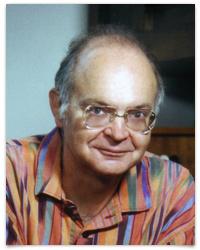
\includegraphics[scale=.5]{images/don_knuth.jpg}
\end{center}
	\caption{Don Knuth, the inventor of \TeX}
	\label{fig:sample}
\end{figure}

\section{Basic Terminology}
As usual the very basic terminology is briefly explained here. Most probably the explanations here only scratch a surface level. More detailed explanations of terminology goes into chapter~\ref{cha:theoretical-background}.

\section{Related Work and Projects}
Here a survey of other work in and around the area of the thesis is given. The reader shall see that the authors of the thesis know their field well and understand the developments there. Furthermore here is a good place to show what relevance the thesis in its field has.

\section{Structure of the Thesis}
%dsflkjas flaksjfl asdfj as lfjldsajflaksdjf sa dfjlasdkfj sadlfjasdklf als dfj l dfsdfsdfn chapter~\ref{cha:used-technologies} (\nameref{cha:used-technologies}) on page~\pageref{cha:used-technologies} we describe the used technologies.
Finally the reader is given a brief description what (s)he can expect in the thesis. Each chapter is introduced with a paragraph roughly describing its content.
\chapter{Digital Signage & XIBO}
\section{Was ist Digital Signage?}\label{sec:digitalsignage}
Digital Signage, in Deutsch Digitales Schild, hat grundsätzlich die Aufgabe Inhalte die meist auf Plakaten oder Schildern angezeigt werden auf Bildschirmen anzuzeigen. Mithilfe von Digital Signage Systemen, soll das zeit- oder interaktionsgesteuerte Ändern von Inhalten auf den Bildschirmen einfach und übersichtlich gehalten werden siehe Abbildung \ref{img:digitalsignagehtlleonding}. Weiteres bietet Digital Signage ein breites Spektrum an Anwendungsbereichen. Digital Signage ist vor allem im Marketing Bereich ein sehr beliebtes Mittel, um ein neues Produkt oder eine Neuheit zu präsentieren. 

https://de.wikipedia.org/wiki/Digital_Signage#Anwendungsbeispiele:_2017.


\begin{figure}[H]
\centering
\includegraphics[width=1\textwidth]{images/02_XiboGrundlagen/Videowall.JPG}
\caption{Digital Signage in der HTL Leonding}
\label{img:digitalsignagehtlleonding}
\end{figure}

\section{Digital Signage Anwendungen}\label{sec:anwendungedigitalsignage}
Digital Signage hat keine Grenzen und kann vielfältig eingesetzt werden. Viele Konzerne nutzen Digital Signage für Marketing Zwecke, Produkte zu präsentieren oder oft auch nur als Lockmittel.

\section{Was ist XIBO?}\label{sec:xibo}
Das XIBO ist ein Open Source Digital Signage System entwickelt von der Spring Signage LTD. Das XIBO-System besteht aus vielen verschiedenen Komponenten. Das XIBO Paket besteht aus einem klassischen Server-Client Konstrukt. Der Server besteht aus drei Komponenten: das Content Managment System welches mithilfe von ZeroMq bei Änderung der Inhalte diese aktualisieren soll, einer Datenbank und einer Weboberfläche, die es dem Benutzer ermöglichen soll das System zu bedienen.

\section{Weboberfläche des XIBO}\label{sec:webpagexibo}
Das Steuerungszentrum des ganzen Signage System ist die Weboberfläche, die ganz einfach über einen Browser unter der Serveraddresse aufgerufen werden kann. Auf der Willkommensseite sind die wichtigsten Funktionen des Signage Servers dargestellt:

\begin{enumerate}
	\item {\em Kalender:} Mit der Kalender Funktion kann eingetragen werden zu welchem Zeitpunkt, welcher Inhalt, auf welchem Bildschirm angezeigt werden soll. Diese Funktion ist einer der wichtigsten und meist verwendeten. In dem Xibo-Kalender werden auch bereits eingetragene Aktivitäten angezeigt.

\begin{figur}
	\centering
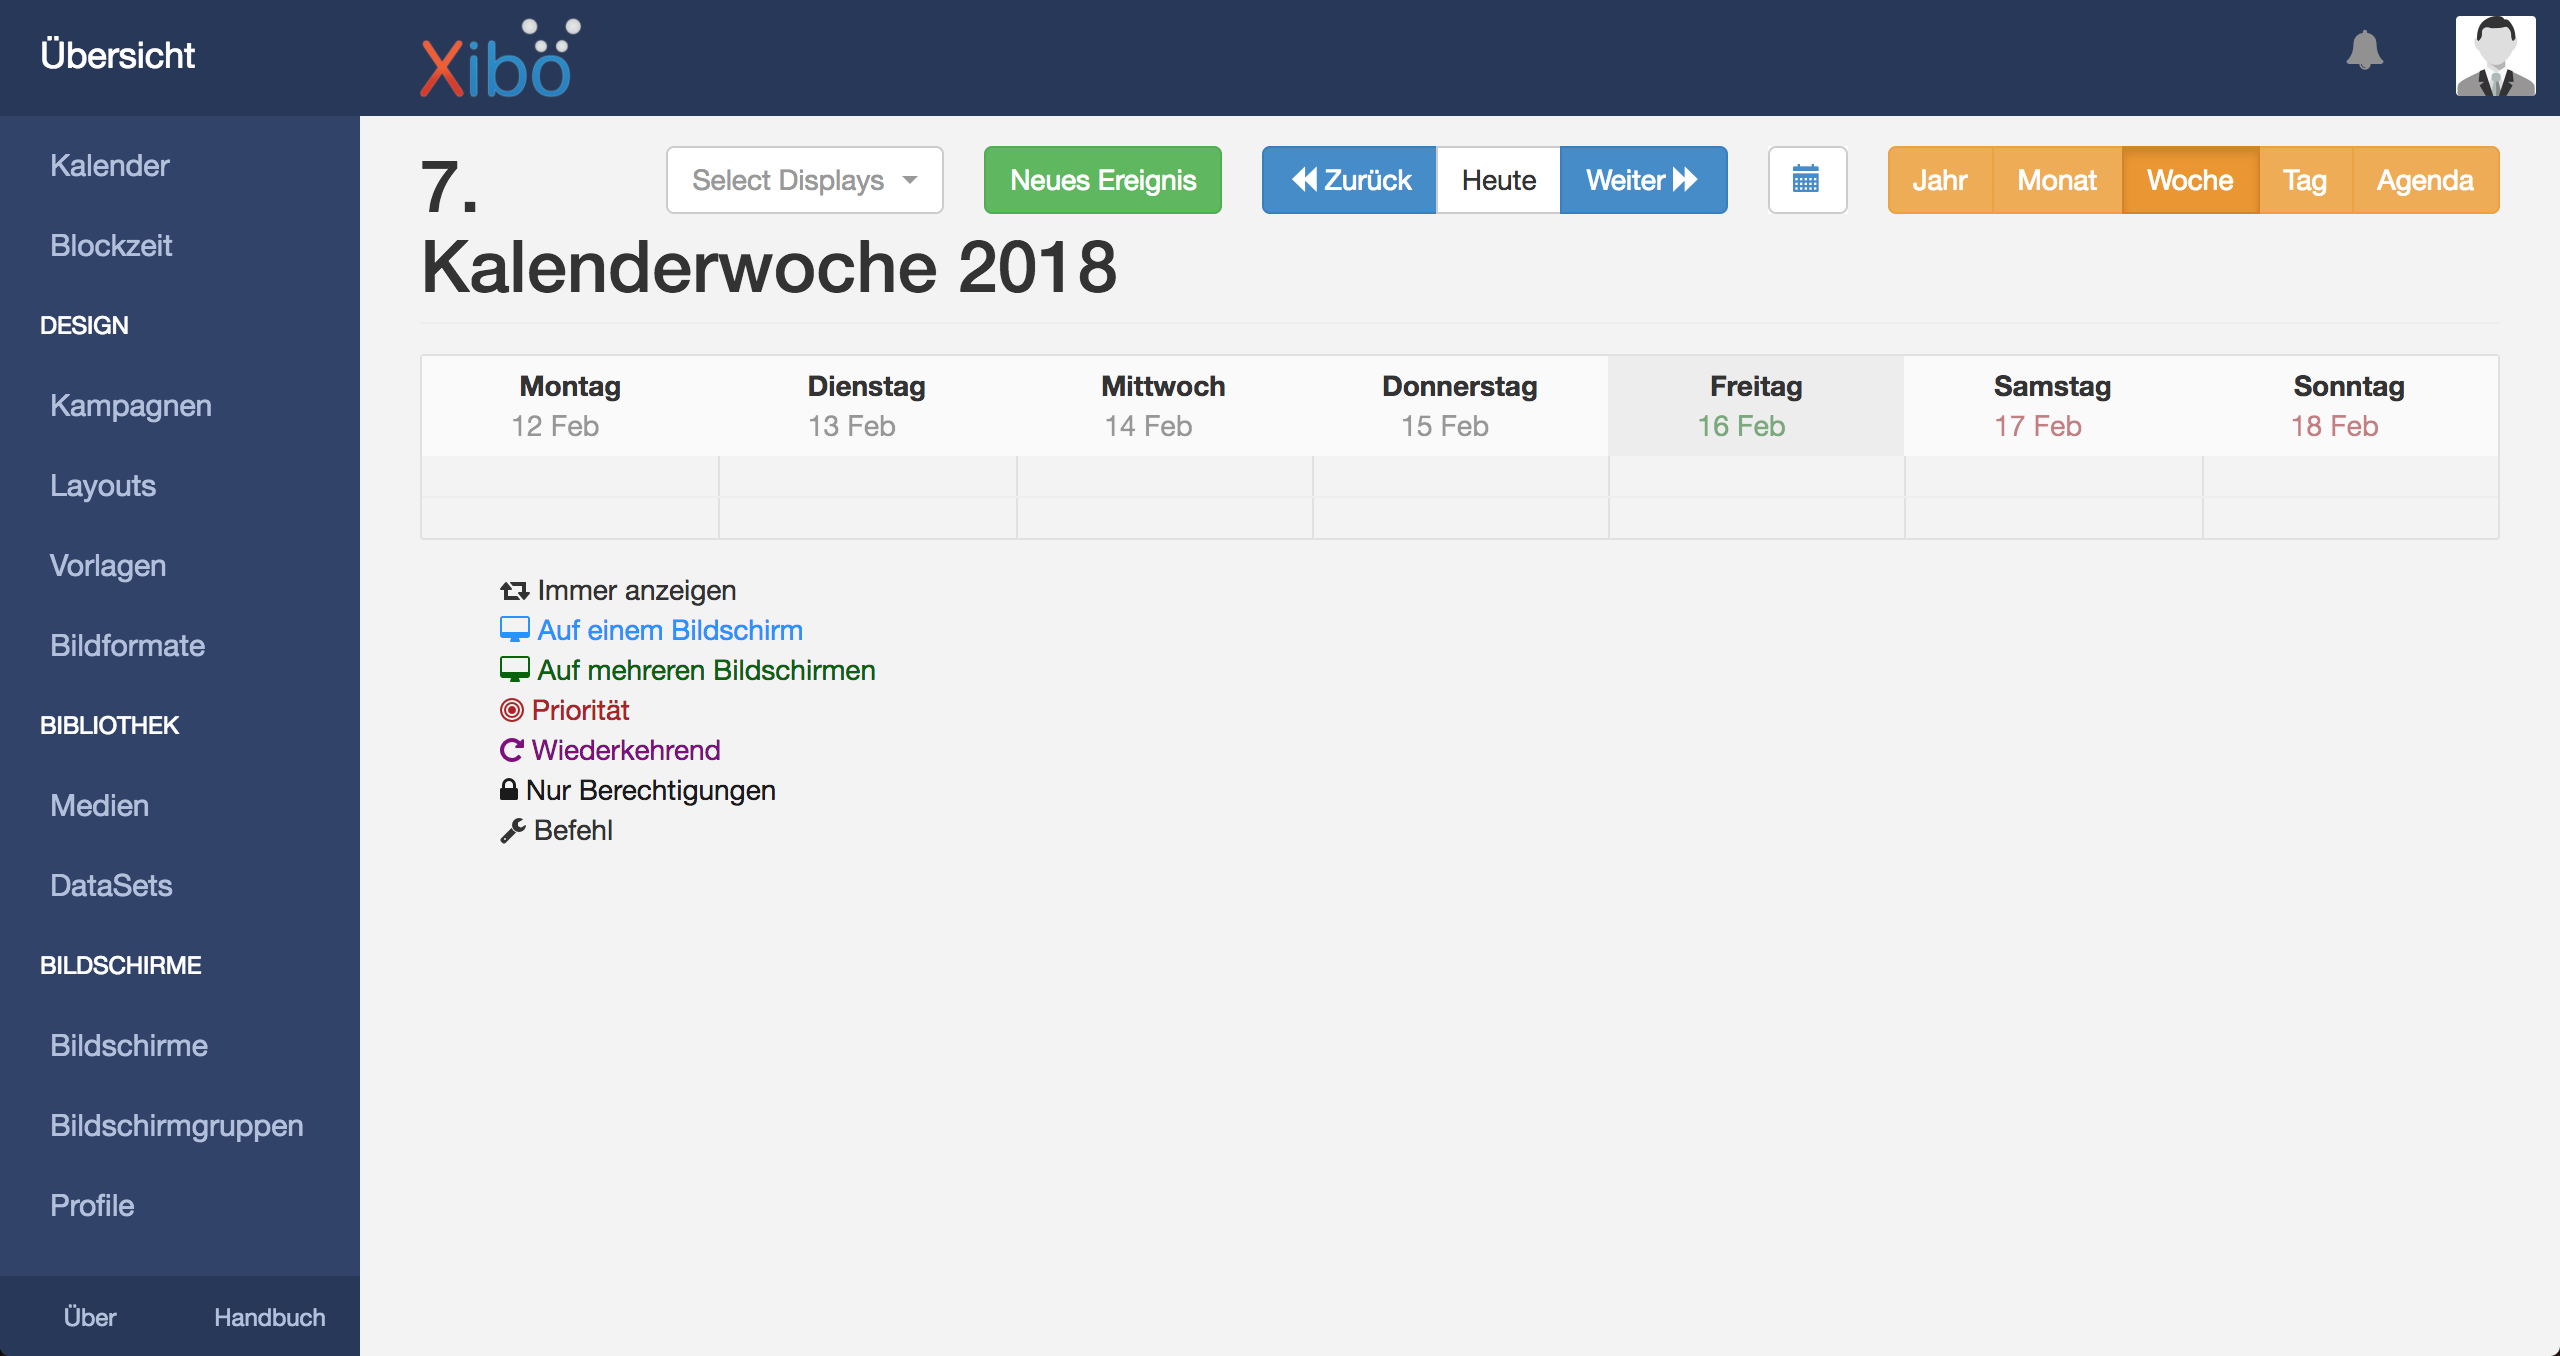
\includegraphics[width=1\textwidth]{images/xibo-basics-calendar}
	\label{img:calendar}
	\caption{XBIO - Kalender}
\end{calendar}	
	
	\item {\em Layouts:} 
	Die Layout-Funktion ist einer der wichtigsten Komponenten des Signage Systems. Es beschäftigt sich mit dem Designen der Inhalte. Auf diese Funktion kommen wir noch einmal zurück.
	
	\item {\em Bibliothek:} 
	Die Bibliothek-Funktion ist zuständig für das Verwalten der Medien. Hier können Sie verschiedene Dateien hochladen.  Diese Medien können dann in Layouts eingebunden und angezeigt werden.
	
	\item {\em Benutzer:} 
	Im Menüpunkt Benutzer können neue Benutzer angelegt und bereits bestehende bearbeitet oder gelöscht werden. Dabei gibt es auch ein Rechte-System. Es können auch Datenmengenbegrenzungen pro Benutzer eingestellt werden.
	
	\item {\em Einstellungen:} 
	Der Menüpunkt Einstellungen gibt dem Nutzer die Möglichkeit, verschiedene Optionen zu wählen. So sind zum Beispiel die richtige Zeitzone, E-Mail Benachrichtigungen, wichtige Einstellungen, die für ein einwandfreies Funktionieren des Xibo-Servers zuständig sind. Aus den Einstellungen ist auch der CMS geheimer Schlüssel zu finden, der für die Authentifizierung der API Zugriffe zuständig ist herauszulesen.
\end{enumerate}

\section{Designen mit XIBO}\label{sec:designexibo}
Beim Designen von einem neuen Layout im XIBO, muss zuerst die Bildschirmauflösung ausgewählt und dem Layout ein passender Name zugewiesen werden, sowie optional auch eine Beschreibung. 

\textbf{Layout Maske}

\begin{calendar}
	\centering
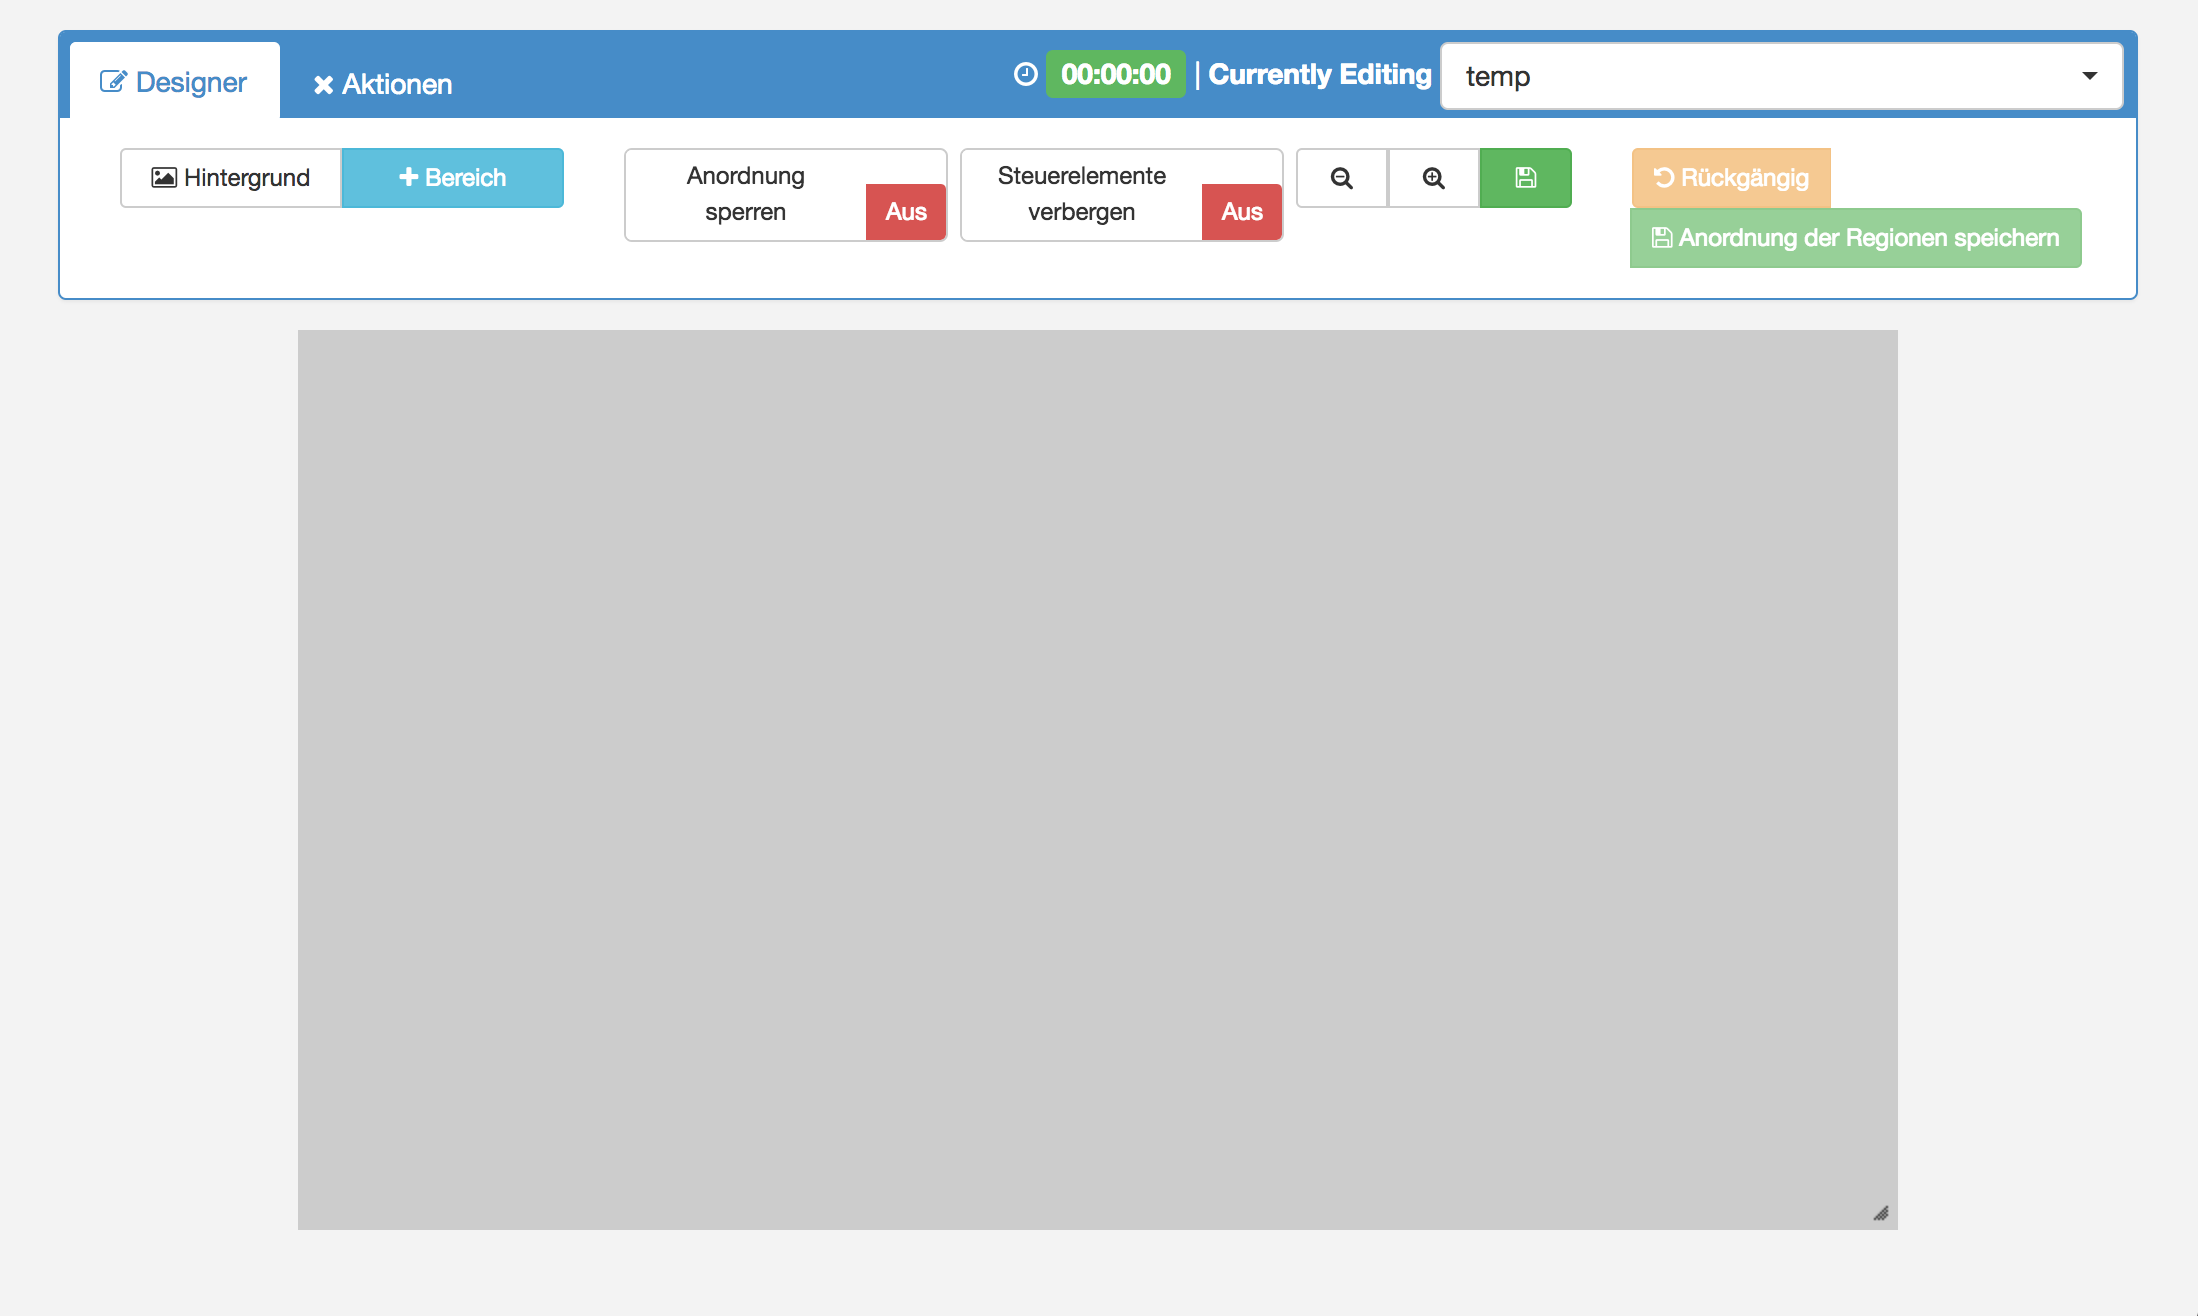
\includegraphics[width=1\textwidth]{images/xibo-basics-designer}
	\label{img:designeLayout}
	\caption{XIBO-Layout designen}
\end{calendar}	

Dem Layout kann nun eine Region oder auch mehrere  hinzugefügt werden. Eine Region kann mehrere Widgets enthalten. Mit einem Doppelklick auf die Region kann ein Widget hinzugefügt werden. Es gibt viele verschiedene Arten von Widgets:

\begin{widgettypes}
	\item {\em Bibliothek:} Mit diesem Widget können Elemente aus der Medienbibliothek in der Region angezeigt werden. Dabei werden PowerPoint Formate, Video, Bilder und andere Medien Datentypen unterstützt.
	
	\item {\em Uhr:} 
	Dieser Widgettyp bindet eine Uhr in die Region ein. Es kann entweder eine Uhr im Analogen Stil oder Digitalen Stil ausgewählt werden.
	
	\item {\em DataSet:} 
	Das DataSet Widget ist sehr wichtig und zeigt grob gesagt nacheinander Daten aus einem Array mit Key, Value Paaren an.
	
	\item {\em Wheather:} 
	Das Wheather Widget, in Deutsch Wetter, zeigt das aktuelle Wetter an. Es kann eingestellt werden ob es anhand von den GPS-Daten des Bildschirmes die Wetterdaten anzeigen soll oder ein vorher definierter Ort für die Daten verwendet werden soll.
	
	\item {\em Flash:} 
	Mit dem Flash Widget können Flash Inhalte abgespielt werden.
	
	\item {\em HLS:} 
	Mit dem HLS Widget können HLS Video Streams angezeigt werden.
	
	\item {\em Image:} 
	Mit dem Image Widget können Bilder entweder aus der XIBO Bibliothek angezeigt oder neue hochgeladen werden.
	
	\item {\em Local Video:} 
	Mit dem Local Video Widget können Videos oder Streams angezeigt werden.
	
	\item {\em PDF:} 
	Mit dem PDF Widget können PDFs entweder aus der XIBO Bibliothek angezeigt oder neue hochgeladen werden.
	
	\item {\em PowerPoint:} 
	Mit dem PowerPoint Widget können PowerPoint Präsentationen entweder aus der XIBO Bibliothek angezeigt oder neue hochgeladen werden.

	\item {\em Text:} 
	Mit dem Text Widget können Texte angezeigt werden.
	
	\item {\em Ticker:} 
	Mit dem Ticker Widget können Texte animiert angezeigt werden. Dabei können diese Texte aus einem DataSet oder einem RSS Feed stammen.
	
	\item {\em Webpage:} 
	Mit dem Webpage Widget können Webseiten angezeigt werden.
\end{widgettypes}

Nachdem eines der Widgets erstellt wurde kann das Ergebnis des Layouts mit einer Layout Vorschau kurz überprüft werden.

\chapter{XIBO-Server}
\section{Beschreibung}
Als zentrale Steuereinheit wird ein XIBO-Server verwendet. Der XIBO-Server bietet die benötigten Funktionalitäten wie zum Beispiel:
\begin{itemize}
	\item {\em Medieninhalte abspielen} 
	\item {\em Zeitsteuerung der anzuzeigenden Informationen}  
	\item {\em Verteilung der Anzeigedaten an die verbundenen Clients} 
\end{itemize}
Es gibt zwei Möglichkeiten den Funktionsumfang des XIBO-Servers zu nutzen. Zum einen über das Server interne Web-Interface, die andere Möglichkeit ist es den Server über die eingebaute REST-Schnittstelle anzusprechen.
\cite{xibo-server}
\section{API}
Die API des XIBO-Servers ist mittels Swagger dokumentiert. Diese Dokumentation deckt die Grundfunktionalitäten und die Form der Anfragen ab. Die Schnittstelle des Servers dient als wesentliches Verbindungsstück zwischen der eigens entwickelten Steuerungssoftware und dem XIBO-Server. Wie der XIBO-Server die verschiedenen Anfragen verarbeitet und entgegen nimmt wurde, bevor die Implementierung des Java-EE-Servers begonnen wurde, mittels Postman getestet. Diese Vorgehensweise war Nötig um festzustellen ob das XIBO-System über REST-API ausreichend konfigurierbar und im operativen Betrieb steuerbar ist. Die Anfragen an den Server wurden im Java Code durch die ''libary'' OkHttp3 übernommen.

\cite{swagger}
\cite{postman}
\cite{Okhttp3}
\section{Authentifizierung}

Die Authentifizierung einer Client-Applikation per REST-Anfrage am XIBO-Server erfolgt über OAuth2 , also mittels Access Token.

Zunächst ist am XIBO-Server ein ''Application''-Objekt im Webinterface zu erstellen. Beim erstellen des ''Application''-Objekts können die Berechtigungen für den Client festgelegt werden. Nachdem das Objekt erstellt wurde stellt dieses ein ''Client Secret'' zur Verfügung. Dieses ist für jeden Client eindeutig. 

Damit ein externer Client auf den XIBO-Server per REST-Request zugreifen beziehungsweise Anweisungen an diesen geben kann, wird ein POST-Request mit folgenden Parametern abgesetzt.

Die Parameter: 
\begin{itemize}
	\item {\em Client\_ID:} XIBO-Server Anwendungen neue Anwendung
	\item {\em Client\_Secret:}  XIBO-Server Anwendungen neue Anwendung
	\item{\em grant\_type:} Muss in der Form ''&grant\_type=client\_credentials''
\end{itemize}

Die über den POST-Request erhaltene Antwort liefert einen Access Token welcher 60 Minuten gültig ist und nach Ablauf erneuert werden muss um weiter über die API zu kommunizieren.
Dieser Token muss bei jedem Request an den XIBO-Server im Header des Requests übergeben werden damit der XIBO-Server feststellen kann ob es sich um einen registrierten Client handelt.

HomeDS\HomeDsBackend\src\main\java\at\htl\utils\AuthentificationHandler.java

Um den die Authentifizierung zu automatisieren wurde eine Java Klasse entwickelt. Funktionsweise dieser wird nachfolgend geschildert: 

Um eine Verbindung zum XIBO-Server herstellen zu können wird eina URL und eine HttpURLConnection deklariert. Im Anschluss wird die URL mit der richtigen Adresse belegt. Die httpURLConnection wird über den Befehl ''httpURLConnection.openConnection()'' dazu angewiesen eine Verbindung aufzubauen. Durch die Anweisung ''httpURLConnection.setDoOutput(true)'' wird der Connection mitgeteilt das als Antwort Daten erhalten werden. Die Art der Anfrage wird als POST-Request festgelegt. Um die für die Authentifizierung am XIBO-Server geforderten Parameter ''client\_id'', ''client\_secret'' und ''grant\_type'' übergeben zu können wird ein ''DataOutputStream'' deklariert und mit dem Benötigten werten versehen. Anschließend werden über den Befehl  ''DataoutputStrem.flush'' wird dem ''DataOutputStream'' mitgeteilt, dass er die Daten über die Verbindung senden soll.Um auftretende Fehler besser finden zu können werden der Übergeben Request-Body, die URL über die der Request durchgeführt wurde und der erhaltene Response-Code im Log-Fenster ausgegeben. Die Daten die anschließend vom XIBO-Server als Antwort erhalten werden, werden durch einen ''BufferedReader'', dieser bekommt bei der Instanziierung den ''InputStream'' der ''httpURLConnection'' übergeben, entgegengenommen. Solange vom Server Daten erhalten werden wird über einen ''StringBuilder'' ein String um jene erhaltenen Daten erweitert. Im Anschluss wird die ''BufferedReader'' Verbindung geschlossen und der erhaltene ''Access\_Token'' wird im Log-Fenster angezeigt. Als nächstes wird der erhaltene Token per ''return'' Statement als Ergebniss der Methode übergeben. Abschließend wird im ''finally'' Block überprüft ob die ''HttpURLConnection'' noch geöffnet beziehungsweise vorhanden ist, sollte dies der Fall sein so wird die Verbindung geschlossen.







\chapter{Verwendente Technologien}
\section{Git und GitHub}
Um dynamisch als Team arbeiten zu können, verwenden wir Software zur Versionsverwaltung. Hierbei handelt es sich um Git. 
Github ist die verwendete Online-Plattform, auf der Benutzer ihre Projekte gratis als Repository speichern. Dies ermöglicht einfaches arbeiten im Team und verhindert in den meisten Fällen Zusammenführungskonflikte. Mittels Git lässt sich auch leicht zurückverfolgen welches, Teammitglied welche Änderungen gemacht hat und im Notfall ist es auch möglich diese Änderungen wieder rückgängig zu machen.

Verwendet wird GitHub für die gesamte Diplomarbeit, sowohl für die Versionierung der Dokumente, als auch  die einzelnen Applicationen. Um sicherzustellen, das keine Konflikte durch paralleles arbeiten entstehen, wird in Branches gearbeitet. Diese Branches wurden erstellt, wenn ein neues Arbeitspaket begonnen wurde, zum Beispiel die Android-App.

Bild Github und verweis Git/GitHub

\section{Android}

Android ist ein Betriebssystem für mobile Endgeräte, spezialisiert für Touch-Anwendungen. Ziel ist es das Endgerät möglichst intuitiv und flexibel bedienen zu können. Mit Android ist es möglich open-source Applicationen zu erstellen die ein großes Publikum erreichen. Google stellt auch einen Markt zur Verfügung in dem die Applicationen gratis oder auch gegen Entgelt erworben werden können.
Diese Aspekte: open-source, gratis und großes Publikum, waren ausschlaggebend dafür, dass die Applicationen in Android implementiert wurden. Als Programmiersprache wurde JAVA verwendet.




\section{Java Enterprise Edition}\label{sec:javaee}
Java Platform, Enterprise Edition oder abgekürzt auch Java EE ist die technische nähere Beschreibung einer Softwarearchitektur, die programmierte Java Anwendungen ausführt.
(weiter ausführen)

QUELLE: https://de.Wikipedia.org/wiki/Java_Platform,_Enterprise_Edition
\chapter{Android Application}
\section{Einleitung}
Um eine höchst mögliche Reichweite an Endgeräten zu erzielen wurde eine Android Application entwickelt, mit der man 



% create further tex files for all other chapters of your document
\chapter{Summary}
Here you give a summary of your results and experiences. You can add also some design alternatives you considered, but kicked out later. Furthermore you might have some ideas how to drive the work you accomplished in further directions.



\bibliography{da_bibliography}{}
\bibliographystyle{alphaurl} % save alternatives are abbrvurl	alphaurl	plainurl	unsrturl

\listoffigures
\listoftables
\chapter*{Project Log Book}
\begin{tabular}{|l|l|l|l|}
\hline
Date & Participants & Todos & Due\\
\hline
\end{tabular}

\appendix
\chapter{Additional Information} \label{cha:additional-information}
If needed the appendix is the place where additional information concerning your thesis goes. Examples could be:
\begin{itemize}
	\item Source Code
	\item Test Protocols
	\item Project Proposal
	\item Project Plan
	\item Individual Goals
	\item \ldots
\end{itemize}
Again this has to be aligned with the supervisor.
\chapter{Individual Goals} \label{cha:individual-goals}
This is just another example to show what content could go into the appendix.
\end{document}  